\documentclass[submit]{harvardml}

% Put in your full name and email address.
\name{David Hughes}
\email{davidralphhughes@college.harvard.edu}

% List any people you worked with.
\collaborators{%
    Alexander Munoz
}

% You don't need to change these.
\course{CS181-S18}
\assignment{Assignment \#5}
\duedate{11:59pm April 18, 2018}
\newcommand{\attr}[1]{\textsf{#1}}
\usepackage[OT1]{fontenc}
\usepackage[colorlinks,citecolor=blue,urlcolor=blue]{hyperref}
\usepackage[pdftex]{graphicx}
\usepackage{subfig}
\usepackage{fullpage}
% \usepackage{palatino}
% \usepackage{mathpazo}
\usepackage{amsmath}
\usepackage{amssymb}
\usepackage{color}
\usepackage{todonotes}
\usepackage{listings}
\usepackage{common}
\usepackage{bm}
\usepackage{enumitem}
\usepackage{tikz}
\usepackage{xifthen}

\usepackage[mmddyyyy,hhmmss]{datetime}

\definecolor{verbgray}{gray}{0.9}

\lstnewenvironment{csv}{%
  \lstset{backgroundcolor=\color{verbgray},
  frame=single,
  framerule=0pt,
  basicstyle=\ttfamily,
  columns=fullflexible}}{}

\newcommand{\mueps}{\mu_{\epsilon}}
\newcommand{\sigeps}{\sigma_{\epsilon}}
\newcommand{\mugam}{\mu_{\gamma}}
\newcommand{\siggam}{\sigma_{\gamma}}
\newcommand{\muzp}{\mu_{p}}
\newcommand{\sigzp}{\sigma_{p}}
\newcommand{\gauss}[3]{\frac{1}{2\pi#3}e^{-\frac{(#1-#2)^2}{2#3}}}


\begin{document}
\begin{center}
{\Large Homework 5: Graphical Models, MDPs}\\
\end{center}

\subsection*{Introduction}

There is a mathematical component and a programming component to this homework.
Please submit your \textbf{tex, PDF, and Python files} to Canvas, and push all
of your work to your GitHub repository. If a question requires you to make any
plots, please include those in the writeup.

\newpage

\section*{Bayesian Networks [7 pts]}
\begin{problem}
  ~

  \noindent In this problem we explore the conditional independence properties
  of a Bayesian Network.  Consider the following Bayesian network representing
  a person's skin condition. Each random variable is binary (true/false).

%\vspace{0.2in}
\begin{center}
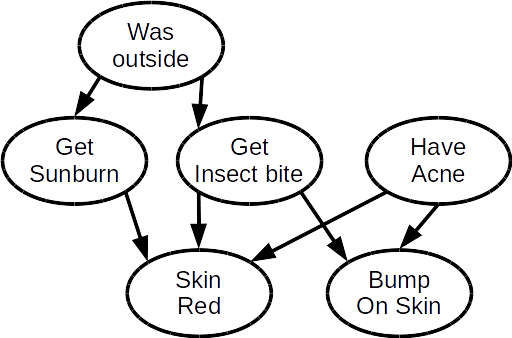
\includegraphics[width=3in]{bn.png}
\end{center}
%\vspace{0.2in}

The random variables are:
%
\begin{itemize}
\item \attr{Was Outside}: Was the person outside?
\item \attr{Get Sunburn}: Did the person get sunburn?
\item \attr{Get Insect Bite}: Did the person get an insect bite?
\item \attr{Have Acne}: Does the person have acne?
\item \attr{Skin Red}: Is the skin red?
\item \attr{Bump on Skin}: Is there a bump?
\end{itemize}

\medskip

For the following questions, $I(A,B)$ means that events A and B are independent
and $I(A,B | C)$ means that events A and B are independent conditioned on C.
Use the concept of d-separation to answer the questions and show your work.


\begin{enumerate}
\item Is $I(\attr{Have Acne},\attr{Was Outside})$? If NO, give
intuition for why.


\item Is $I(\attr{Have Acne},\attr{Was Outside}\given \attr{Skin Red})$? If NO,
    give intuition for why.


\item Is $I(\attr{Get Sunburn},\attr{Bump on Skin})$? If NO, give intuition for
    why.

\item Is $I(\attr{Get Sunburn},\attr{Bump on Skin}\given \attr{Get Insect
    Bite})$? If NO, give intuition for why.

\item Suppose the person has taken a medicine to suppress their response to
    insect bites: they get red skin, but no bumps.  Draw the modified network.


\item For this modified network, is $I(\attr{Get Sunburn},\attr{Bump on
    Skin})$? If NO, give an intuition why.  If YES, describe what observations
    (if any) would cause them to no longer be independent.

\end{enumerate}
\end{problem}

\subsection*{Solution}
\begin{enumerate}
    \item
        Yes they are independent.
    \item
        No, they are not independent. If skin is red and have acne, there is a
        decreased probability of outside.
    \item
        No, not independent. Having a sunburn increases the chances of being
        outside, which increases the chances of having an insect bite, and
        increases the probability of getting a bump on the skin.
    \item
        Yes, independent.
    \item \text{} \\
        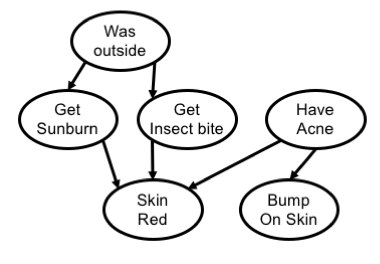
\includegraphics[scale=.5]{bn2.png}
    \item
        Yes independent. If we observe skin red, they'd no longer be
        independent because having red skin and getting sunburned would
        decrease the probability of acne, and decrease the probability of a
        bump on the skin.
\end{enumerate}

\newpage

\section*{Kalman Filters [7 pts]}

\begin{problem}
  In this problem, you will implement a one-dimensional Kalman filter.
  Assume the following dynamical system model:
  \begin{eqnarray*}
    z_{t+1} &= z_{t} + \epsilon_{t} \\
    x_{t} & = z_{t} + \gamma_{t}
  \end{eqnarray*}
  where $z$ are the hidden variables and $x$ are the observed
  measurements.  The random variables $\epsilon$ and $\gamma$ are
  drawn from the following Normal distributions:
  \begin{eqnarray*}
    \epsilon_t &\sim& N(\mueps,\sigeps) \\
    \gamma_t &\sim& N(\mugam,\siggam)
  \end{eqnarray*}
  where $\mueps = 0$, $\sigeps=0.05$, $\mugam = 0$ and $\siggam=1.0$

  You are provided with the observed data $x$ and the hidden data $z$ in
  kf-data.csv, and the prior on the first hidden state is $p(z_0)$ =
  N($\muzp$,$\sigzp$) where $\muzp = 5$ and $\sigzp=1$


    \begin{itemize}
      \item[(a)] The distribution $p(z_t|x_0...x_t)$ will be Gaussian
          $N(\mu_t,\sigma^2_t)$. Derive an iterative update for the mean
          $\mu_t$ and variance $\sigma^2_t$ given the mean and variance at the
          previous time step ($\mu_{t-1}$ and  $\sigma^2_{t-1}$).

       \item[(b)] Implement this update and apply it to the observed data above
           (do not use the hidden data to find these updates). Provide a plot
           of $\mu_t$ over time as well as a $2\sigma_t$ interval around
           $\mu_t$ (that is $\mu_t \pm 2\sigma_t$).  Does the Kalman filter
           ``catch up'' to the true hidden object?

       \item[(c)] Repeat the same process but change the observation at time
           $t=10$ to $x_{t=10}=10.2$ (an extreme outlier measurement).  How
           does the Kalman filter respond to this outlier?

       \item[(d)] Comment on the misspecification of dynamical system model for
           these data.  Based on the previous two parts, how does this
           misspecification affect the predictions?

\end{itemize}
\end{problem}

\subsection*{Solution}
\begin{enumerate}
    \item Complete the square to integrate:
        \begin{align*}
            p(z_t|z_{t-1}) &\sim N(z_{t-1},\sigma_{\epsilon}) \\
                p(x_t|z_t) &\sim N(z_t,\sigma_{\gamma}) \\
            p(z_t|x_{0:t}) &= \int_{z_{t-1}}
                              p(z_t|z_{t-1,x_{0:t}})dz_{t-1} \\
                           &= p(x_t|z_t) \int_{z_Pt-1}p(z_t|z_{t-1})
                              p(z_{t-1}|x_{0:(t-1)})dz_{t-1} \\
                           &\propto \int
                              \exp\bigg(-\frac{1}{2\sigma_\epsilon^2}(z_t -
                              z_{t-1})^2 -
                              \frac{1}{2\sigma_\gamma^2}(x_t-z_t)^2 -
                              \frac{1}{2\sigma_{t-1}^2}
                              (\overline{z}_{t-1}-z_{t-1})dx_{t-1} \bigg) \\
                           &= \exp\bigg(-\frac{1}{2}\bigg(z_t^2
                              \bigg(\frac{1}{\sigma_\gamma^2} +
                              \frac{1}{\sigma_\epsilon^2 + \sigma_{t-1}^2}
                              \bigg) - 2z_t
                              \bigg(\frac{\overline{x}_{t-1}}{\sigma_\epsilon^2
                              + \sigma_{t-1}^2} + \frac{x_t}{\sigma_\gamma^2}
                              \bigg) \bigg) \bigg)
        \end{align*}
        The updates are:
        \begin{align*}
            \overline{z}_t &= \overline{z}_{t-1} + \frac{\sigma_\epsilon^2 +
                              \sigma_{t-1}^2}{\sigma_\epsilon^2
                              + \sigma_{t-1}^2 + \sigma_\gamma^2}(x_t -
                              \overline{z}_{t-1}) \\
                \sigma_t^2 &= \sigma_\gamma^2 \frac{\sigma_\epsilon^2 +
                              \sigma_{t-1}^2}{\sigma_\epsilon^2
                              + \sigma_{t-1}^2 + \sigma_\gamma^2}
        \end{align*}

    \item
        The Kalman filter does catch up to the true hidden object. \\
        \begin{center}
            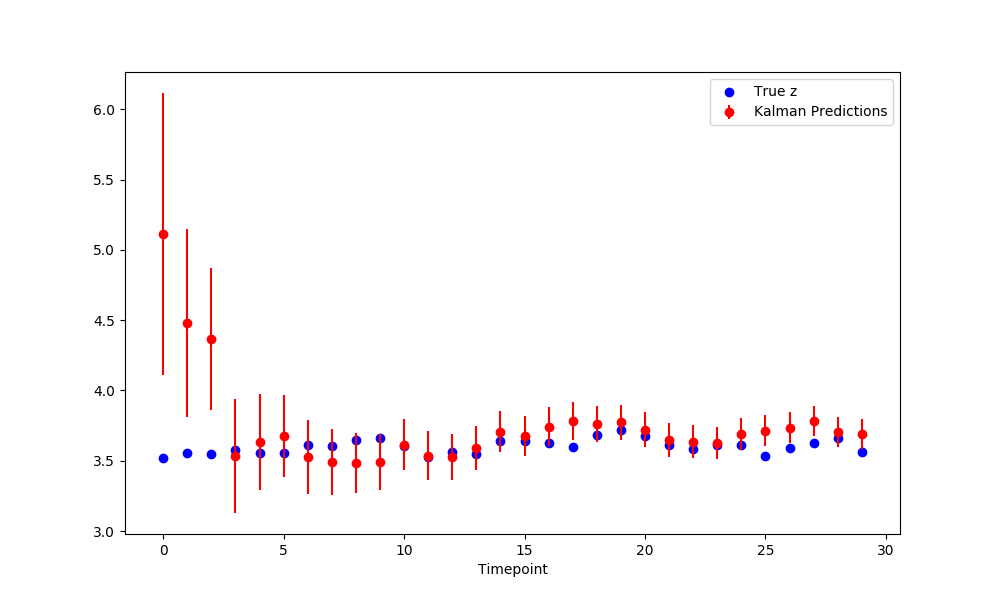
\includegraphics[scale=0.6]{kalman1.png}
        \end{center}
    \item
        The Kalman filter is drastically affected by the single outlier. \\
        \begin{center}
            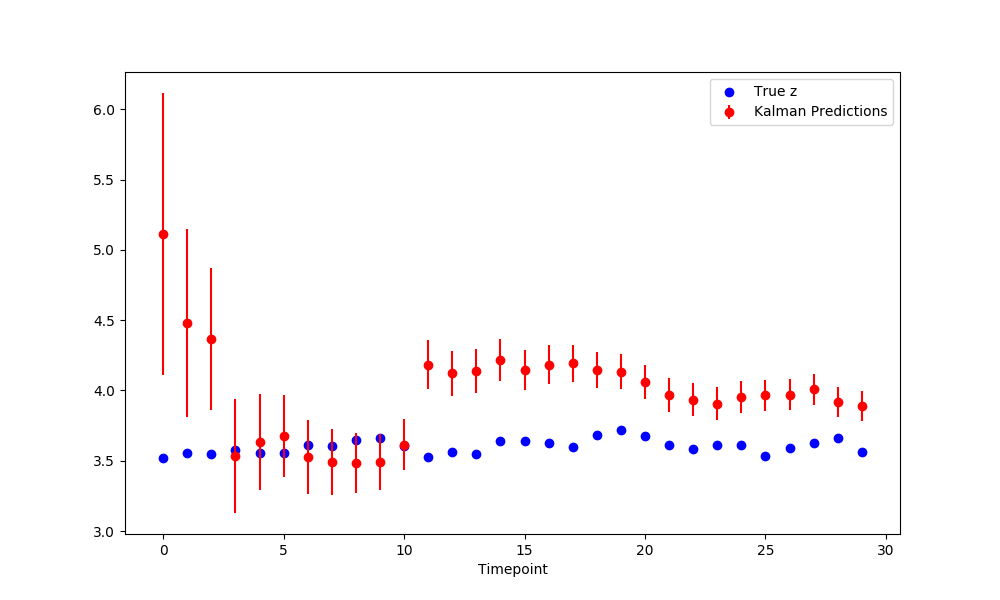
\includegraphics[scale=0.6]{kalman2.png}
        \end{center}
    \item
        The model is mis-specified because the single outlier drastically
        affects the Kalman filter predictions, however the error bars do not
        account for this change. Looking at the formulae for the updates in
        part 2, we can see the fraction determines the power of the update: the
        larger this fraction, the more we will update based on new
        observations. We tune increasing $\sigma_\gamma$ to rely less on the
        new update and decrease sensitivity to outliers.
\end{enumerate}

\newpage

\section*{Markov Decision Processes [7 pts]}
\begin{problem}
  ~


  \noindent In this problem we will explore the calculation of the \emph{MDP
  value function} $V$  in a 2D exploration setting, without time discounting
  and for a finite time horizon.

Consider a robot navigating the following grid:\\
  \begin{center}
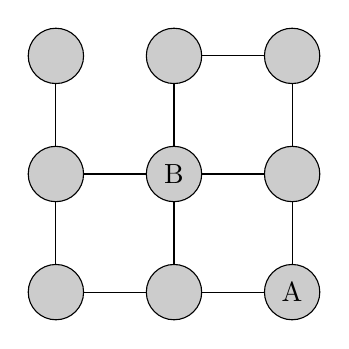
\begin{tikzpicture}[darkstyle/.style={circle,draw,fill=gray!40,minimum size=20}]
  \foreach \x in {0,...,2}
    \foreach \y in {0,...,2}
       {\node [darkstyle]  (\x\y) at (1.5*\x,1.5*\y) {\ifthenelse{\x=2 \AND \y=0}{A}{\ifthenelse{\x=1\AND\y=1}{B}{}}};}

       \draw (00)--(01);
       \draw (01)--(02);

       \draw (10)--(11);
       \draw (11)--(12);

       \draw (10)--(11);
       \draw (11)--(21);

       \draw (20)--(21);
       \draw (11)--(21);

       \draw (21)--(22);
       \draw (01)--(11);
       \draw (00)--(10);
       \draw (12)--(22);

       \draw (10)--(20);

\end{tikzpicture}
\end{center}
The robot moves in exactly one direction each turn (and must move). The robot's
goal is to maximize its score in the game after $T$ steps. The score is defined
in the following way:

\begin{itemize}
  \item If the robot's movement attempts to move it off the grid, then the
      robot loses a point (-1) and stays where it is.
  \item If the robot ends its motion on node A, it receives 10 points, and if
      it moves onto node B, it receives -100 points. Otherwise, it receives 0
      points.
\end{itemize}

  \begin{enumerate}
    \item Model this as a Markov decision process: define the states $S$,
        actions $A$, reward function $r:S\times A\mapsto \mathbb{R}$, and
        transition model $p(s'\given s, a)$ for $s', s\in S$ and $a\in A$.  For
        now, assume that the robot's actions execute perfectly: if the robot
        tries to move in a particular direction, it always succeeds in doing
        so.

    \item Consider a \emph{random policy} $\pi$, where in each state the robot
        moves uniformly at randomly in any of its available directions
        (including off the board).  For every position on the grid calculate
        the value function, $V^\pi_t: S\mapsto \mathbb{R}$, under this policy,
        for $t=2, 1$ steps left to go.  You can find LaTeX code for the tables
        in the solution template. Note that you should have 2 tables, one for
        each time horizon.

    \item Now assume that the robot plays an \emph{optimal policy} $\pi^\ast_t$
        (for $t$ time steps to go). Find the optimal policy in the case of a
        finite time horizon of $t = 1, 2$ and give the corresponding MDP value
        functions $V^\ast_t: S\mapsto \mathbb{R}$, under this optimal policy.
        You can indicate the optimal policy for each time horizon on the
        corresponding $V^\ast_t$ table via arrows or words in the direction
        that the robot should move from that state.

    \item Now consider the situation where the robot does not have complete
        control over its movement. In particular, when it chooses a direction,
        there is a 80\% chance that it will go in that direction, and a 10\%
        chance it will go in the two adjacent (90$^\circ$ left or 90$^\circ$
        right) directions. Explain how this changes the elements $S$, $A$, $r$,
        and $p(s' \given s,a)$ of the MDP model.  Assume the robot uses the
        same policy $\pi^\ast_t$ from the previous question (now possibly
        non-optimal), and write this as $\pi_t$, and tie-break in favor of N,
        then E, then S then W.  Give the corresponding MDP value functions
        $V^\pi_t: S\mapsto \mathbb{R}$, for this policy in this partial control
        world, for $t=2, 1$ steps left to go. Is the policy still optimal?
  \end{enumerate}
\end{problem}
\subsection*{Solution}
\begin{enumerate}
    \item
        The states $S$ are the 9 different nodes. The actions $A$ are up, down,
        left, and right. The reward function is -1 if the action ends in a
        state off the map, +10 if the action ends in state $A$, -100 if the
        action ends in state $B$, and 0 otherwise. If the action will take you
        off the map, the transition probability is 0, and 1 otherwise.

    \item
        To calculate with one timepoint to go, we average over the
        probabilities:
        $$V_{t=1}^\pi(s) = r(s, \pi(s))$$

        \begin{center}
        \begin{tabular} {| c | c | c |}
            \hline
            -0.75 & -25.5 & -0.5 \\ \hline
            -0.25 & 0 & -22.75 \\ \hline
            -0.5 & -22.75 & -0.5 \\ \hline
        \end{tabular}
        \end{center}

        With two timepoints left, we add the expected current reward with the
        expected future reward:
        $$V_{t=2}^\pi(s)  = r(s,\pi(s)) + \sum_{s' \in
        S}p(s'|s,\pi(s))V_{t-1}^\pi(s') $$

        \begin{center}
        \begin{tabular} {| c | c | c |}
            \hline
            -1.375 & -38.375 & -12.81 \\ \hline
            -0.575 & -17.81 & -28.69 \\ \hline
            -0.65 & -28.69 & -12.13 \\ \hline
        \end{tabular}
        \end{center}

    \item \text{} \\
        \begin{center}
        t=1:
        \begin{tabular} {| c | c | c |}
            \hline
            \downarrow (0) & \rightarrow (0) & \downarrow (0) \\ \hline
            \uparrow (0) & \uparrow (0) & \downarrow (+10) \\ \hline
            \uparrow (0) & \rightarrow (+10) & \uparrow (0) \\ \hline
        \end{tabular} \\

        t=2:
        \begin{tabular} {| c | c | c |}
            \hline
            \downarrow (0) & \rightarrow (0) & \downarrow (+10) \\ \hline
            \uparrow (0) & \rightarrow (+10) & \downarrow (+10) \\ \hline
            \rightarrow (+10) & \rightarrow (+10) & \uparrow (+10) \\ \hline
        \end{tabular}
        \end{center}
    \item
        States $S$, actions $A$, and reward function $r$ would be identical as
        in previous parts. The difference now is in the transition
        probabilities. Specifically, while trying to go from state $s$ to state
        $s'$, there is an 80\% chance of transitioning to $s'$, a 10\% chance
        of transitioning 90 degrees left, and 10\% chance of transitioning 90
        degrees right.

        \begin{center}
        t=1:
        \begin{tabular} {| c | c | c |}
            \hline
            \downarrow (-0.2) & \rightarrow (-10.1) & \downarrow (-0.1) \\ \hline
            \uparrow (-10.1) & \uparrow (0) & \downarrow (-9.1) \\ \hline
            \uparrow (-0.1) & \rightarrow (-9.1) & \uparrow (-0.1) \\ \hline
        \end{tabular} \\

        t=2:
        \begin{tabular} {| c | c | c |}
            \hline
            \downarrow (-9.31) & \rightarrow (-10.41) & \downarrow (-8.4) \\ \hline
            \uparrow (-11.27) & \rightarrow (-9.2) & \downarrow (-10.09) \\ \hline
            \rightarrow (-8.4) & \rightarrow (-10.09) & \uparrow (-8.3) \\ \hline
        \end{tabular}
        \end{center}
\end{enumerate}

\newpage
\begin{problem}[Calibration, 1pt]
Approximately how long did this homework take you to complete? 10 hours
\end{problem}


\begin{itemize}
    \item Name: David Hughes
    \item Email: davidralphhughes@college.harvard.edu
    \item Collaborators: Alexander Munoz
\end{itemize}

\end{document}
